% -*- TeX-master: "User_guide"; fill-column: 75 -*-

\section{SBML packages overview}
\label{sec:extensionsOverview}

In this section, we quickly overview the state of the \SBMLthree packages currently
implemented for JSBML to provide users with documentation of what's possible with SBML and JSBML.
Each package description is accompanied by a 
class hierarchy describing the current state of development for the
package. Note smaller package descriptions correspond to packages in
active standards development, however, packages are up to date
with respect to the latest released standards.

\begin{figure}[hb]
 \centering
 \vspace*{2ex}
 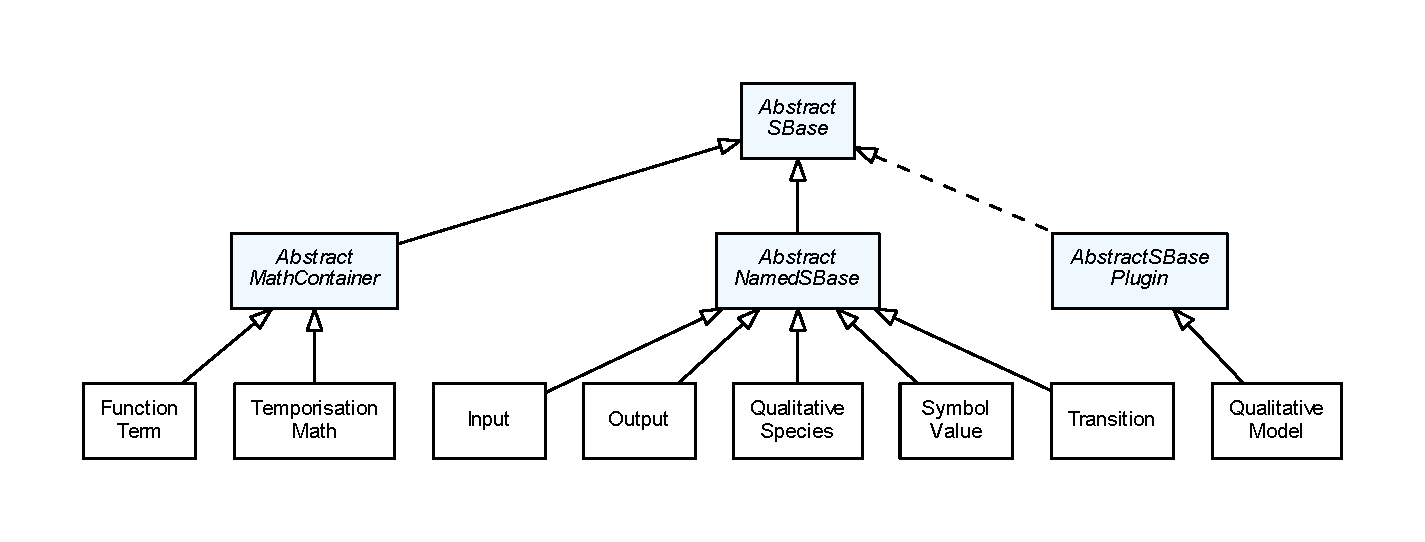
\includegraphics[width=\textwidth]{../../../extensions/qual/doc/img/type_hierarchy.pdf}
 \caption[Class diagram of the qualitative models extension]{Class diagram of the qualitative models extension. Qualitative Models package (\code{qual}, for short) allows species in a model to 
have non-quantitative or non-continuous concentrations \cite{Chaouiya2013}. 
This may manifest as Boolean or discrete values, and is primarily employed in 
modelling gene regulation, signalling pathways, and metabolic networks using 
logical/Boolean networks \cite{shmulevich2002} or Petri nets 
\cite{breitling2008}, which in turn, do not rely on traditional quantitative
coefficients to encode relationships between biochemical entities.}
 \label{fig:qual}
\end{figure}

\begin{figure}[hb]
 \centering
 \vspace*{2ex}
 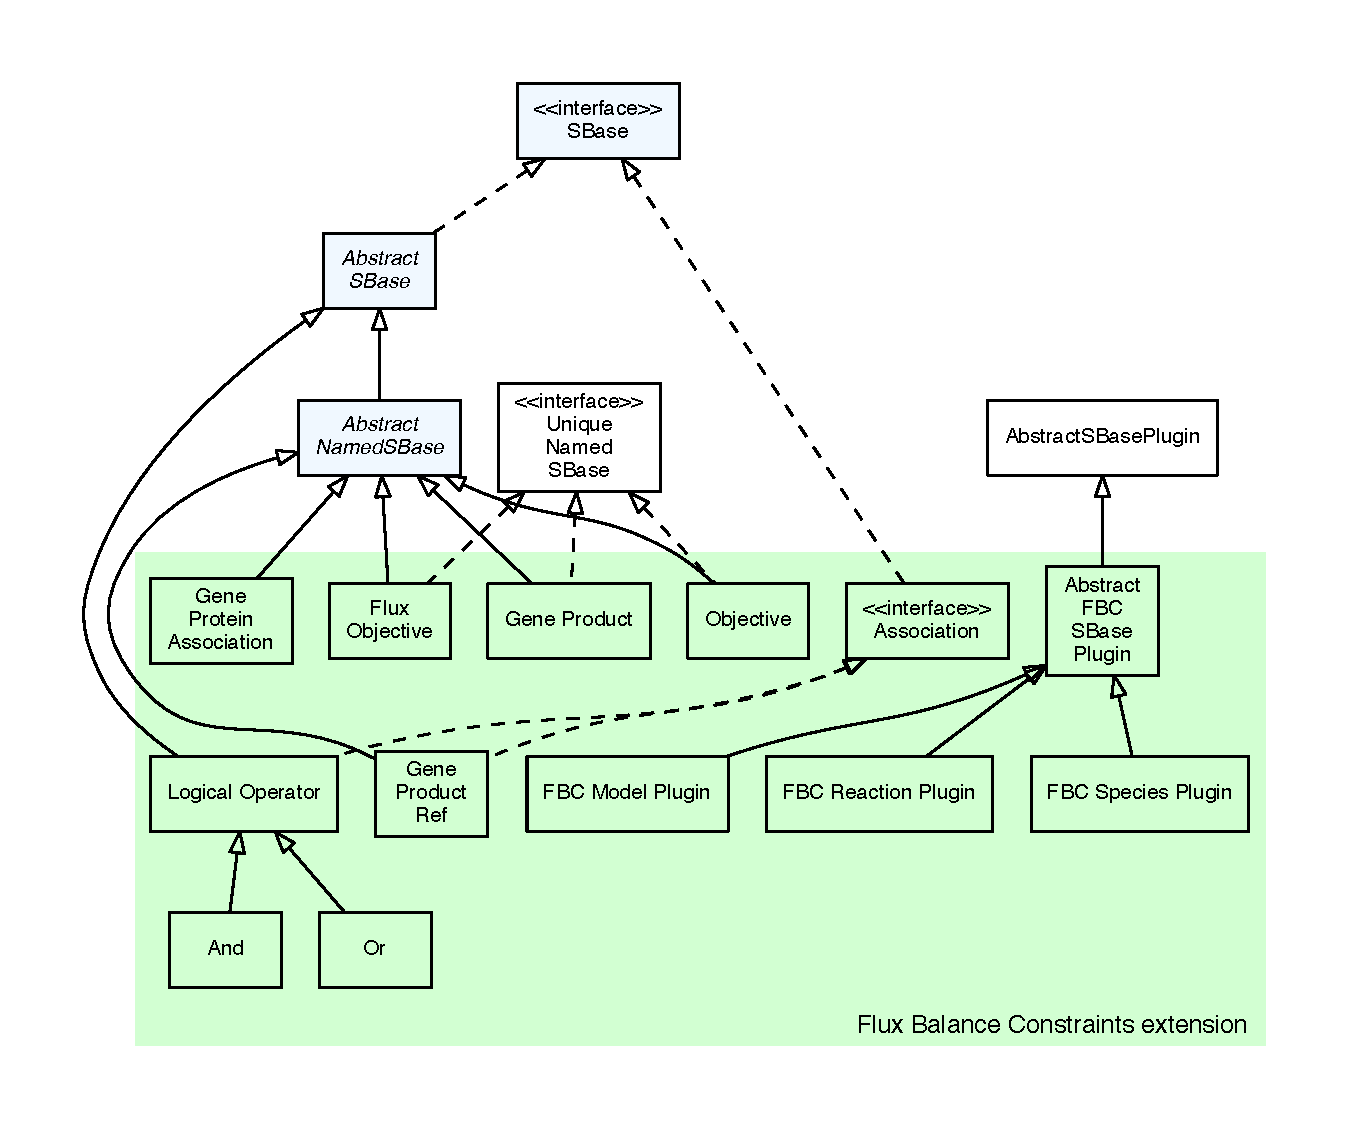
\includegraphics[width=\textwidth]{../../../extensions/fbc/doc/img/type_hierarchy.pdf}
 \caption[Class diagram of the flux balance constraints extension.]{Class diagram of the flux balance constraints extension. Constraints-based modelling \cite{lewis2012} utilizes a class of models in which
the canonical stoichiometric relations between reactions and metabolites are specified
as constraints for convex analysis and mathematical optimization. Although species,
reactions, and stoichiometry can be encoded using the SBML L3V1,
Flux Balance Constraints (\code{fbc}, \cite{olivier2013}) enable a constraints
based perspective. For example, the constraints based approach called
Flux Balance Analysis (FBA) often aims to find the maximum growth rate of the
cell given a set of uptake possibilities and the ratio of molecules needed
for cell growth. The mathematical formulation for this optimization problem
has variables of reaction fluxes and constraints of mass balances around the
metabolites and bounds on the variable reaction fluxes. Because this formulation is
underdetermined, an objective, usually one that maximizes a biomass function which
corresponds to growth rate, is supplied which optimizes the reaction fluxes. Therefore,
the \code{fbc} package extends the SBML Level 3 core to specifically encode for bounds on
fluxes, constraints, and objective functions, which facilitates a fluid interface to
existing constraints-based modelling software and optimization solvers.}
 \label{fig:fbc}
\end{figure}

\begin{figure}[hb]
 \centering
 \vspace*{2ex}
 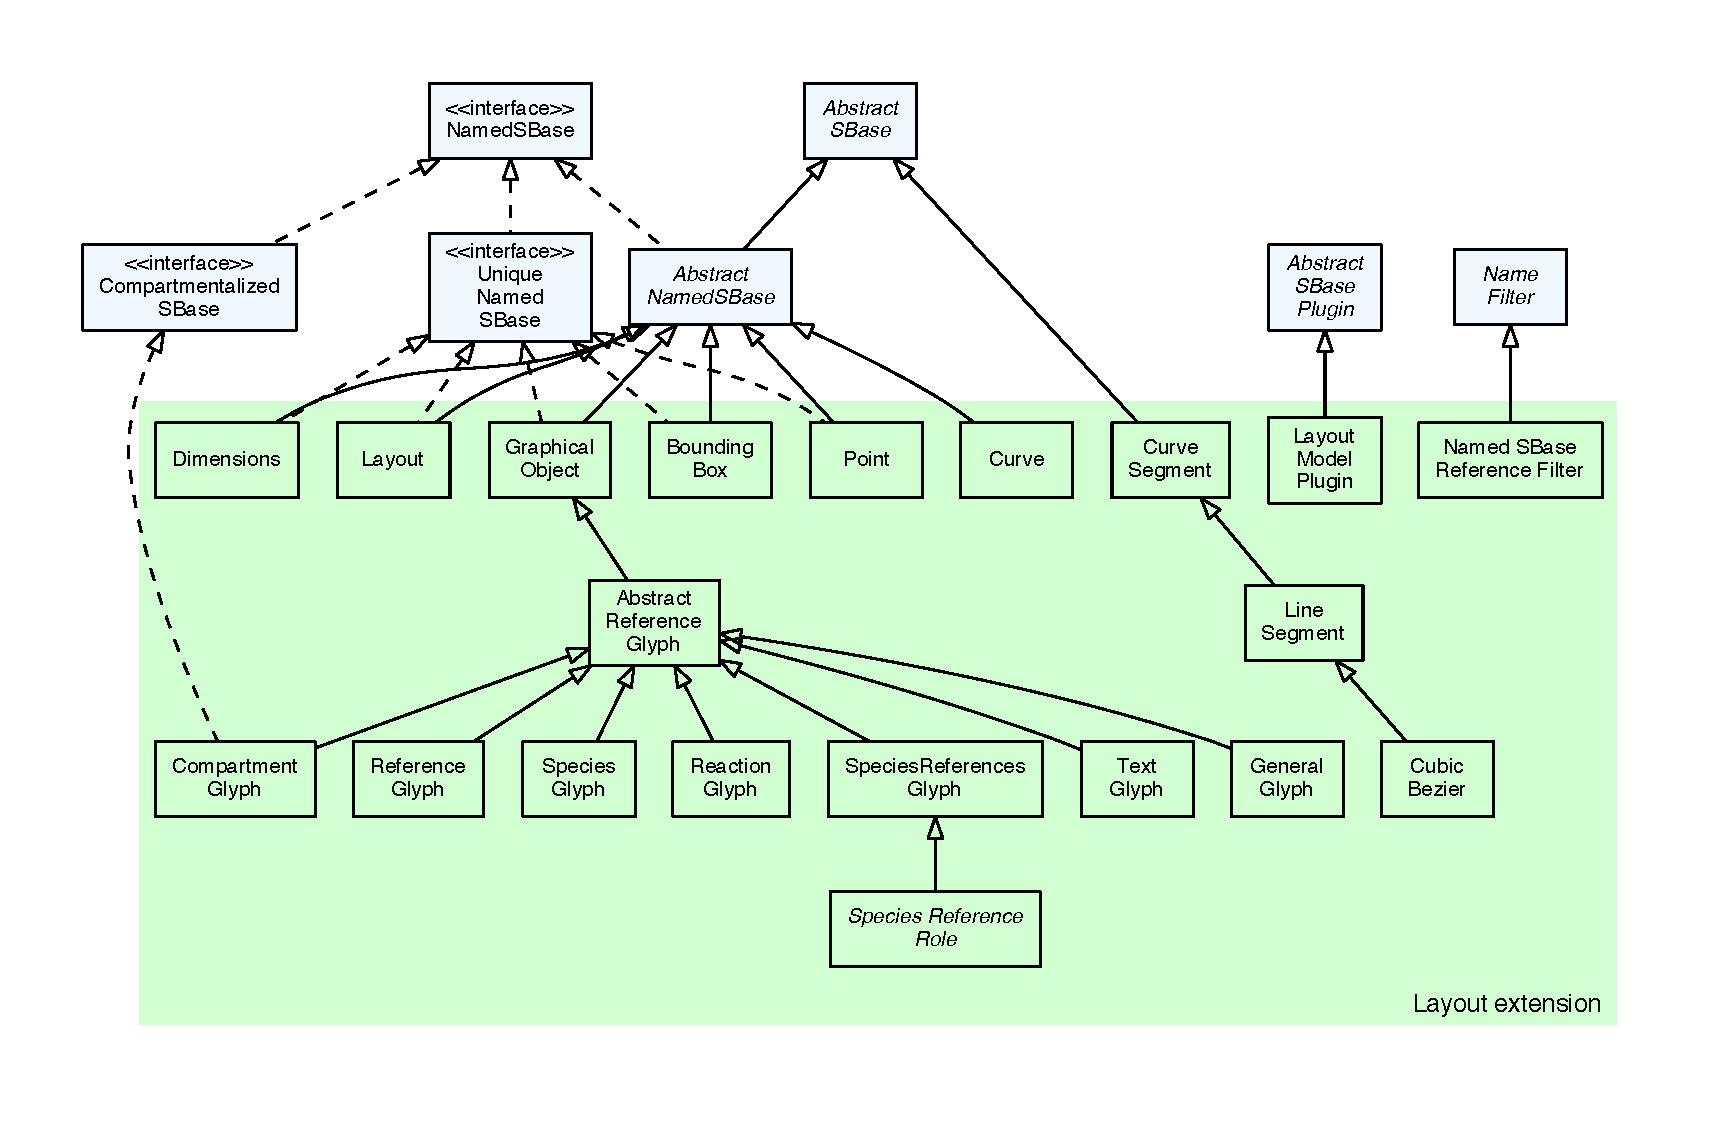
\includegraphics[width=\textwidth]{../../../extensions/layout/doc/img/type_hierarchy.pdf}
 \caption[Class diagram of the layout extension]{Class diagram of the layout extension. SBML encodes a core set of components (species, reactions) that make up
biochemical networks. The \code{layout} extension supports specifying graphical
information for these components. The structure for this extension mirrors 
the SBML Level 3 core hierarchy by introducing graphical object (\code{glyph})
counterparts to reactions and species. Different \code{glyph} types can optionally correspond
to elements in standard SBML, and there can be many \code{glyphs} for one element.
In addition, \code{layout} elements of non-standard model components can be specified
using the generic \code{GraphicalObject} class. Although this extension is powerful
enough to encode the position of all biochemically related graph components,
it should be noted that the scope of this package does not include rendering
of these components. This functionality is provided by the \code{Render} package.
Ultimately, the \code{layout} extension provides a common language that biochemical
graph editors and viewers can utilize to couple a model to a graph layout.}
 \label{fig:layout}
\end{figure}

\begin{figure}[hb]
 \centering
 \vspace*{2ex}
 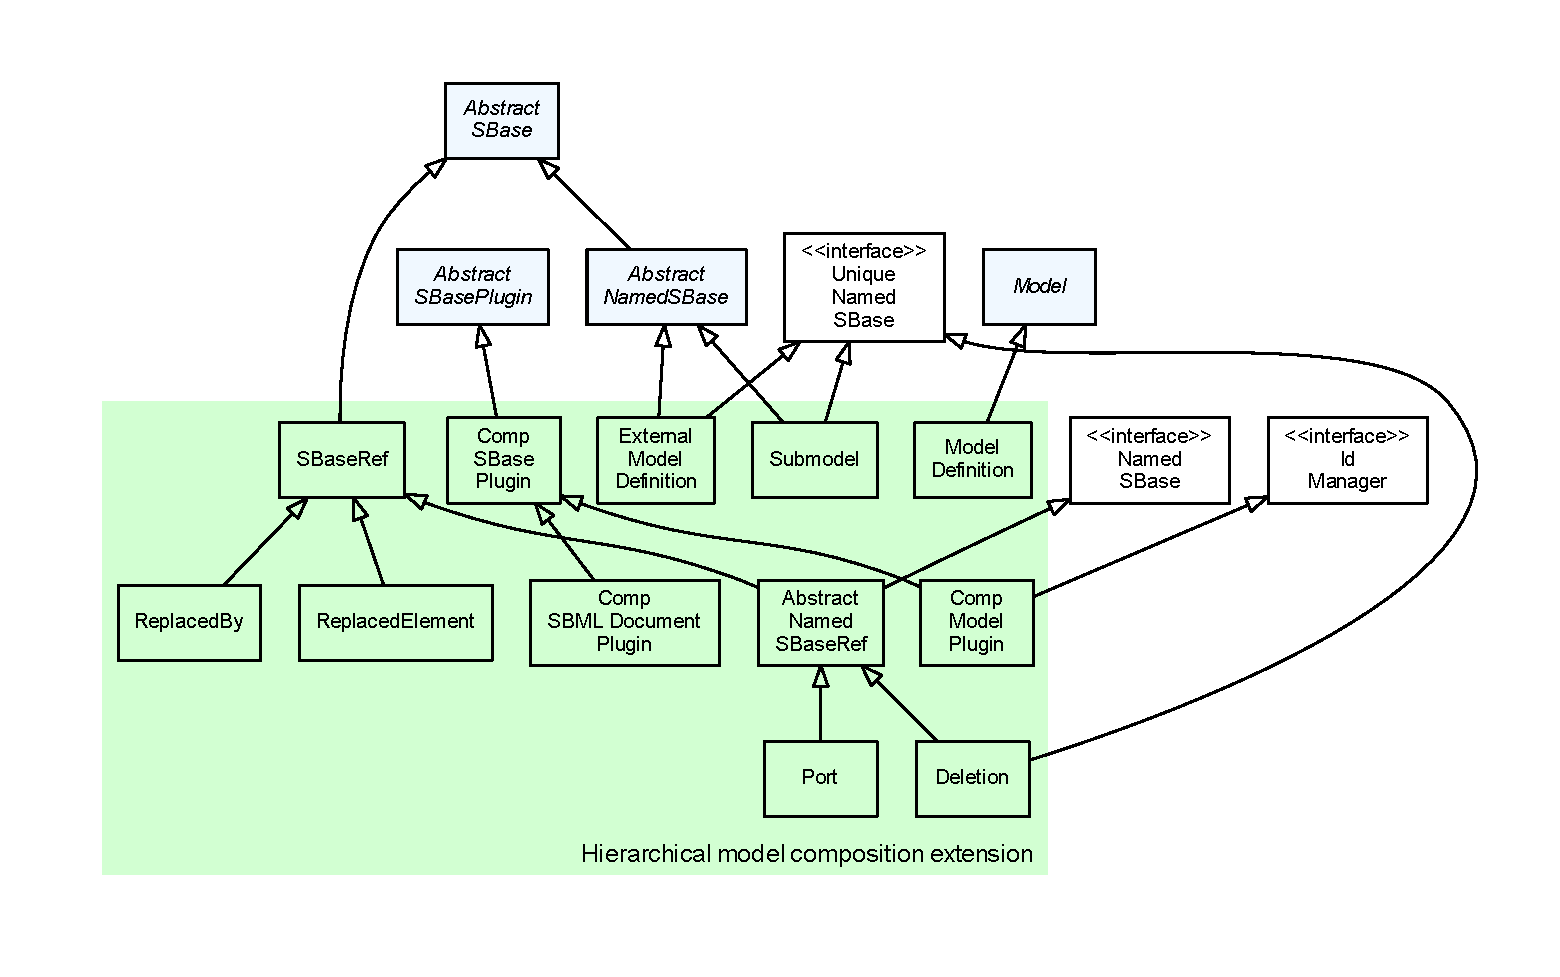
\includegraphics[width=\textwidth]{../../../extensions/comp/doc/img/type_hierarchy.pdf}
 \caption[Class diagram of the hierarchical model composition extension]{Class diagram of the hierarchical model composition extension. As the amount of information for biochemical networks increases, models tend to
increase in complexity as well. The Hierarchical Model Composition extension (\code{comp}; \cite{smith2010})
attempts to contextualize this complexity by providing a generic framework to encode
models as hierarchical entities in an SBML document. This functionality also allows
for storing multiple instances of a model within an enclosing model or document, which
can be used to build libraries of models within a document or to independently manage
different parts of a large model. Classes allow modellers to access elements within
sub-models and interface with other sub-models, and \code{comp} provides a standardized approach
to define sub-model differences with respect to parent or reference models. Overall, \code{comp}
is a powerful extension to the SBML Level 3 core that gives modellers and programmers
options to standardize the encoding of complex, modular modelling frameworks. 
}
 \label{fig:comp}
\end{figure}

\begin{figure}[hb]
 \centering
 \vspace*{2ex}
 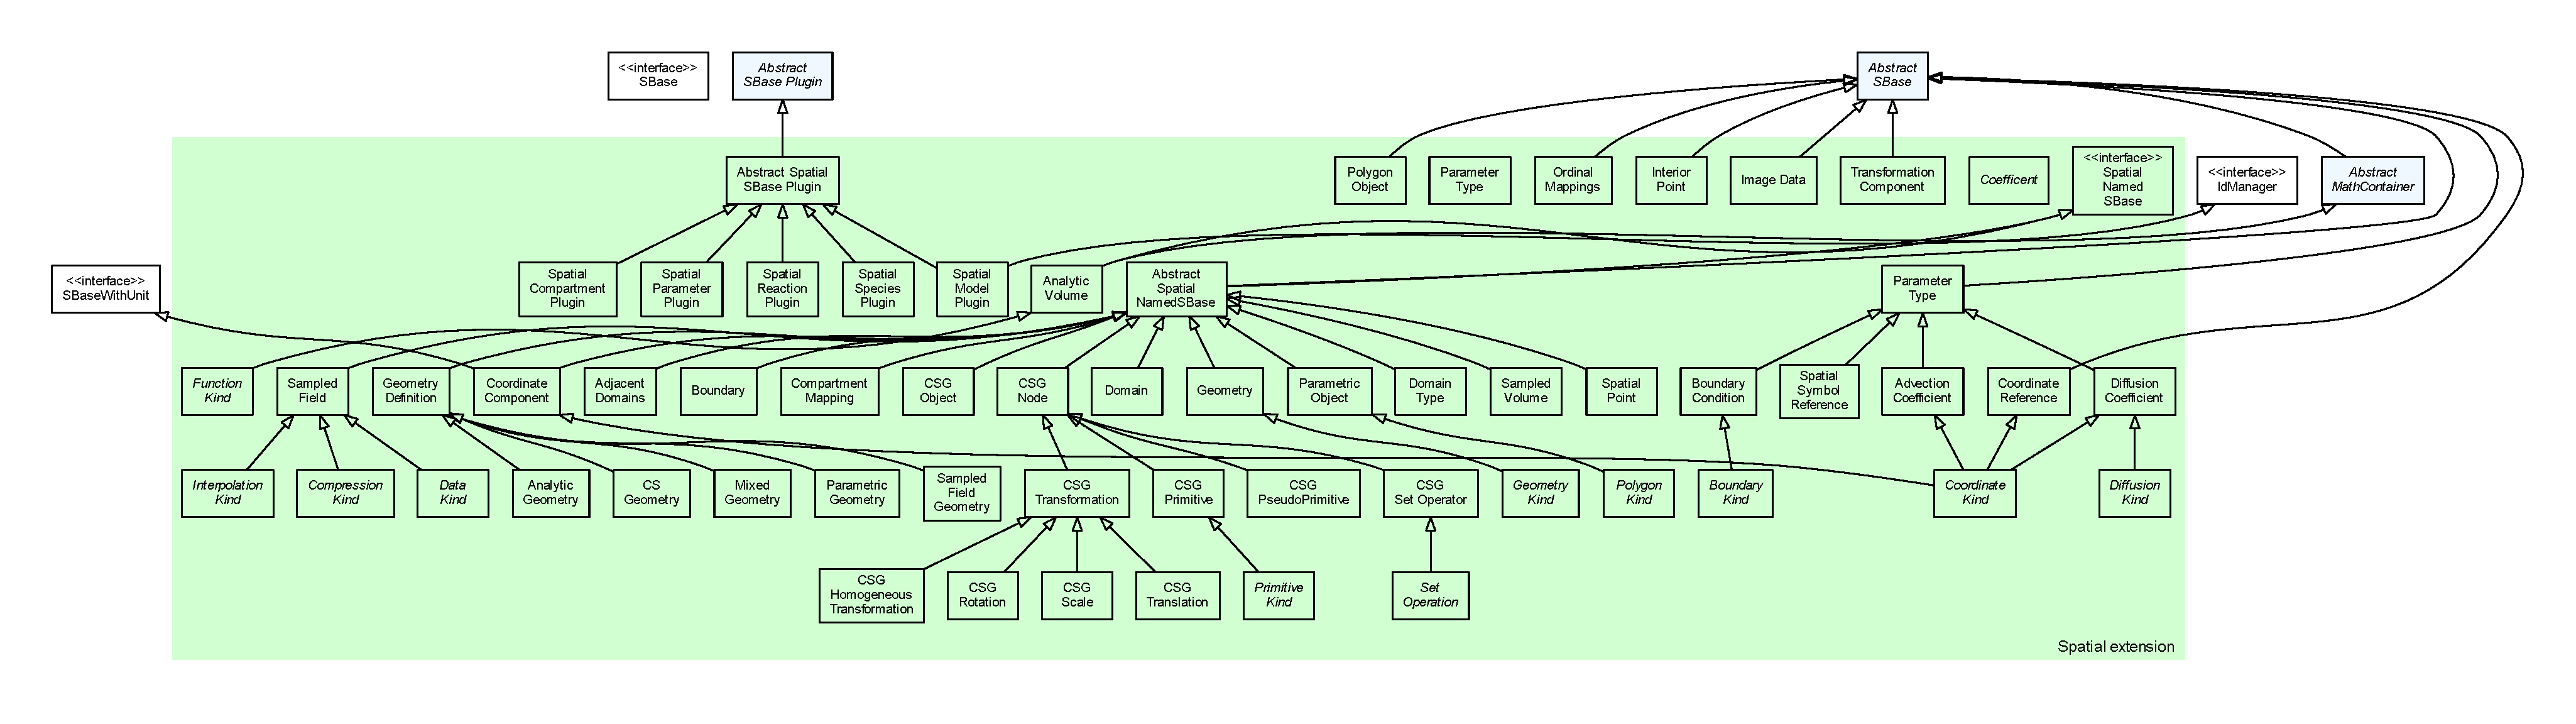
\includegraphics[width=\textwidth]{../../../extensions/spatial/doc/img/type_hierarchy.pdf}
 \caption[Class diagram of the spatial processes extension]{Class diagram of the spatial processes extension. The Spatial Processes extension (\code{spatial}, \cite{Schaff2014})
provides the ability to the SBML Level 3 core to specify subcellular,
geometric locations for components in biochemical
models. Although subcellular locations can be abstractly represented via
compartments in the SBML core specifications, \code{spatial} enables the encoding of
a cellular coordinate system which can describe non-uniform molecular distributions,
diffusive transport, and spatially localized reactions. The \code{Geometry} class holds
the spatial information and the extended \code{Species}, \code{Reaction}, \code{Compartment}, and
\code{Parameter} objects have mappings to the \code{spatial} objects that hold information on
molecular transport coefficients, geometric domains, and coordinates. \code{Spatial} is
therefore able to store the geometric information commonly used in spatial modelling
tools for the biochemical entities from standard SBML.}
 \label{fig:spatial}
\end{figure}

\begin{figure}[hb]
 \centering
 \vspace*{2ex}
 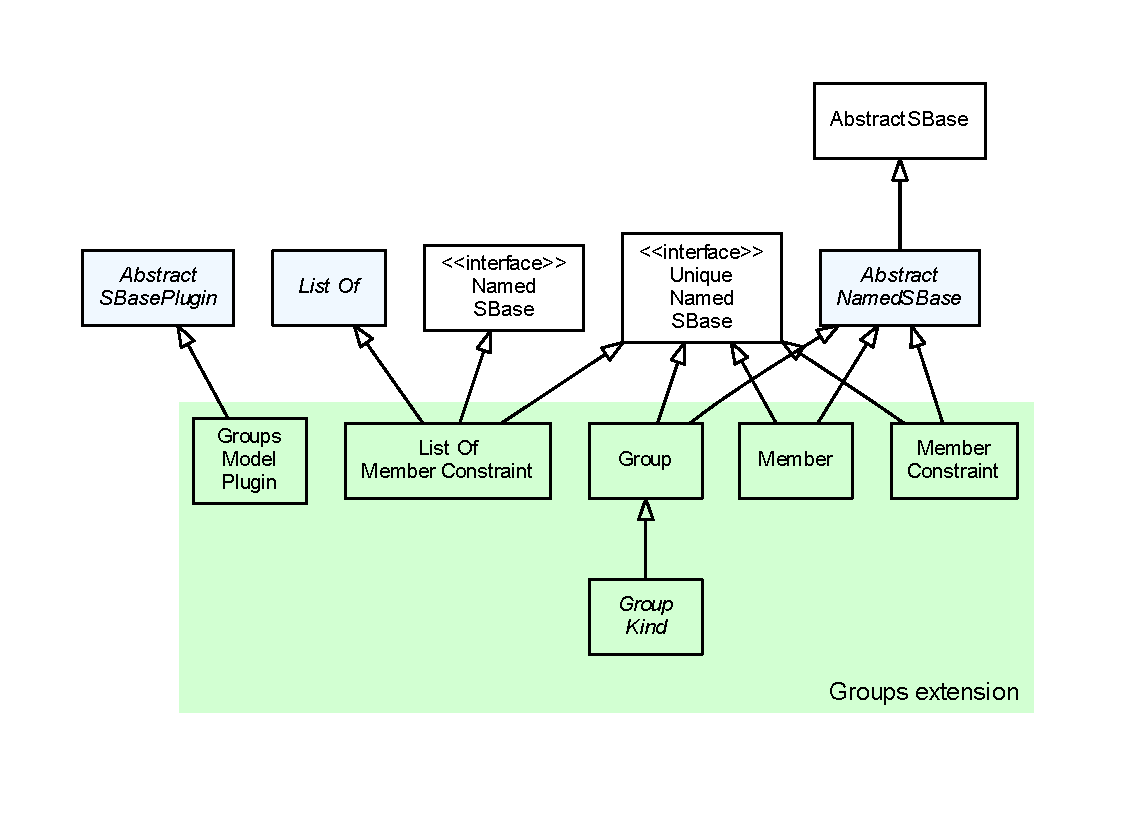
\includegraphics[width=\textwidth]{../../../extensions/groups/doc/img/type_hierarchy.pdf}
 \caption[Class diagram of the groups extension]{Class diagram of the groups extension. \code{Groups} is a simple extension that links together elements in an SBML model. Coupling
\code{groups} information with annotation and SBO terms \cite{Courtot2011a} 
contextualizes these sets of objects for properly conveying roles of groups 
for other programmers and modellers.}
 \label{fig:groups}
\end{figure}


\begin{figure}[hb]
 \centering
 \vspace*{2ex}
 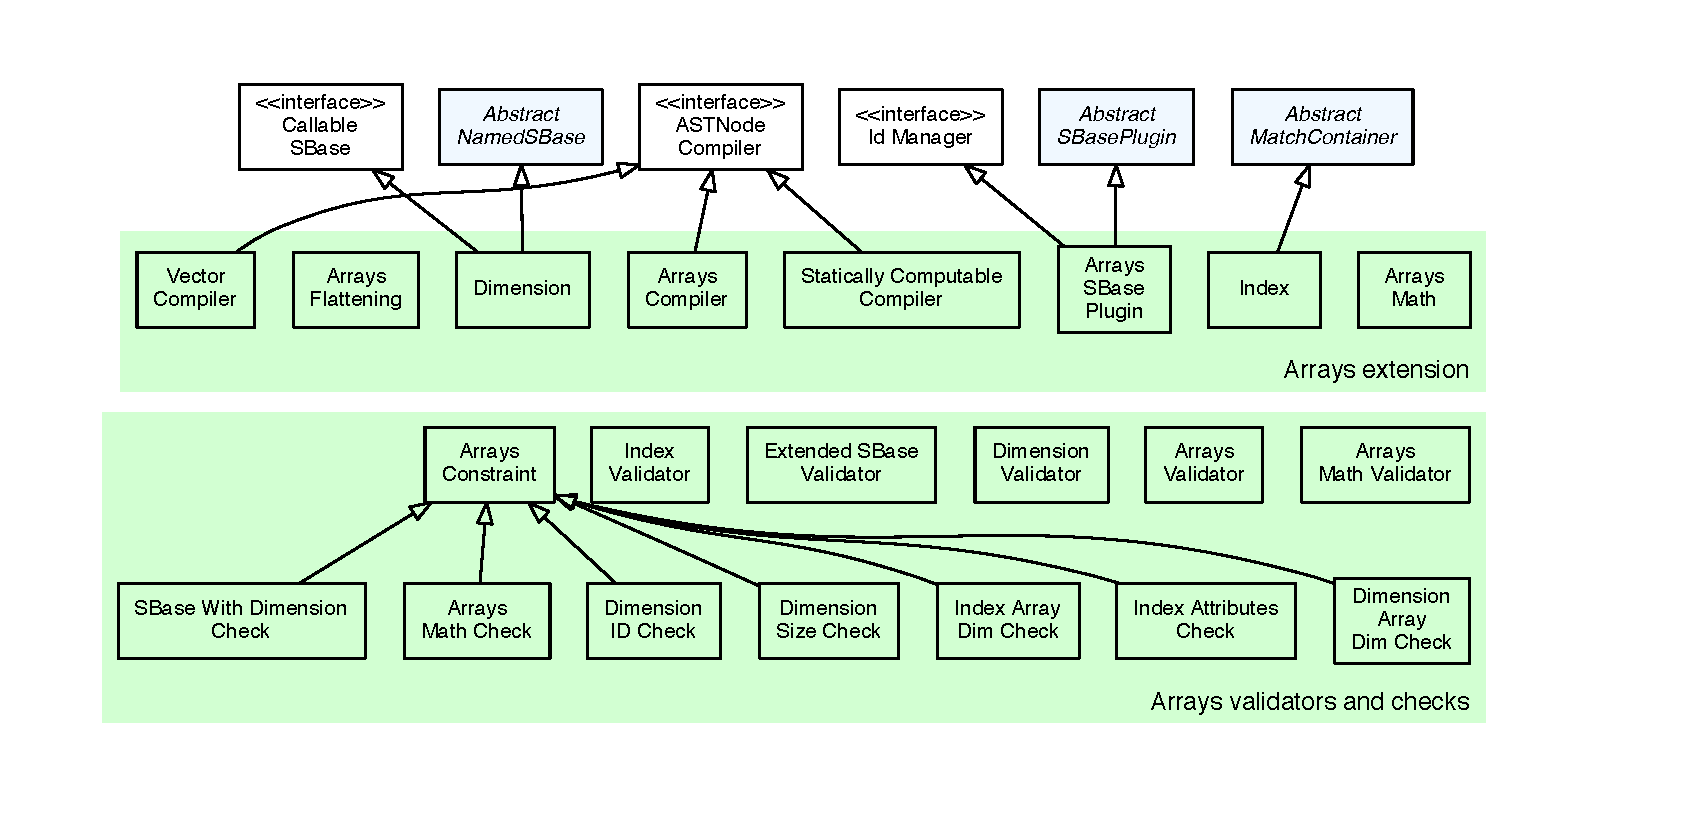
\includegraphics[width=\textwidth]{../../../extensions/arrays/doc/img/type_hierarchy.pdf}
 \caption[Class diagram of the arrays extension]{Class diagram of the arrays extension. Arrays (\code{arrays}, \cite{Watanabe2013}) extends SBML variables to include arrays of values,
thereby representing repeated or regular model structures more efficiently.
\code{Arrays} provides the ability to access sets of values with indices instead of explicit
declaration and creation of sub-data objects.}
 \label{fig:arrays}
\end{figure}


\begin{figure}[hb]
 \centering
 \vspace*{2ex}
 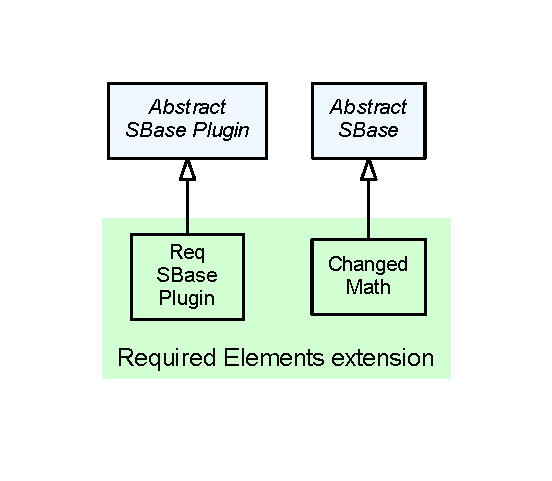
\includegraphics[width=.5\textwidth]{../../../extensions/req/doc/img/type_hierarchy.pdf}
 \caption[Class diagram of the required elements extension]{Class diagram of the required elements extension. Required Elements (\code{req}, \cite{Smith2013}) allows a model to indicate which
components have had their mathematical meanings changed by (e.g.) the use of
another SBML package.}
 \label{fig:arrays}
\end{figure}


\begin{figure}[hb]
 \centering
 \vspace*{2ex}
 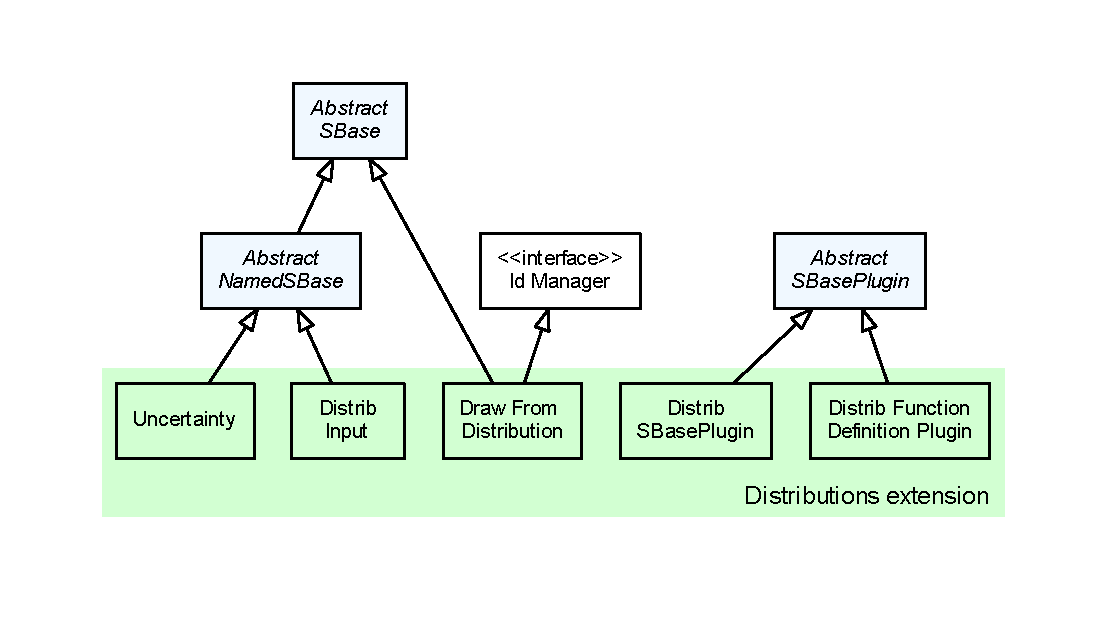
\includegraphics[width=\textwidth]{../../../extensions/distrib/doc/img/type_hierarchy.pdf}
 \caption[Class diagram of the distributions extension.]{ Class diagram of the distributions extension. Distributions 
 (\code{distrib}, \cite{Moodie2013}) encodes statistical distributions and their sampling.}
 \label{fig:distrib}
\end{figure}

\begin{figure}[hb]
 \centering
 \vspace*{2ex}
 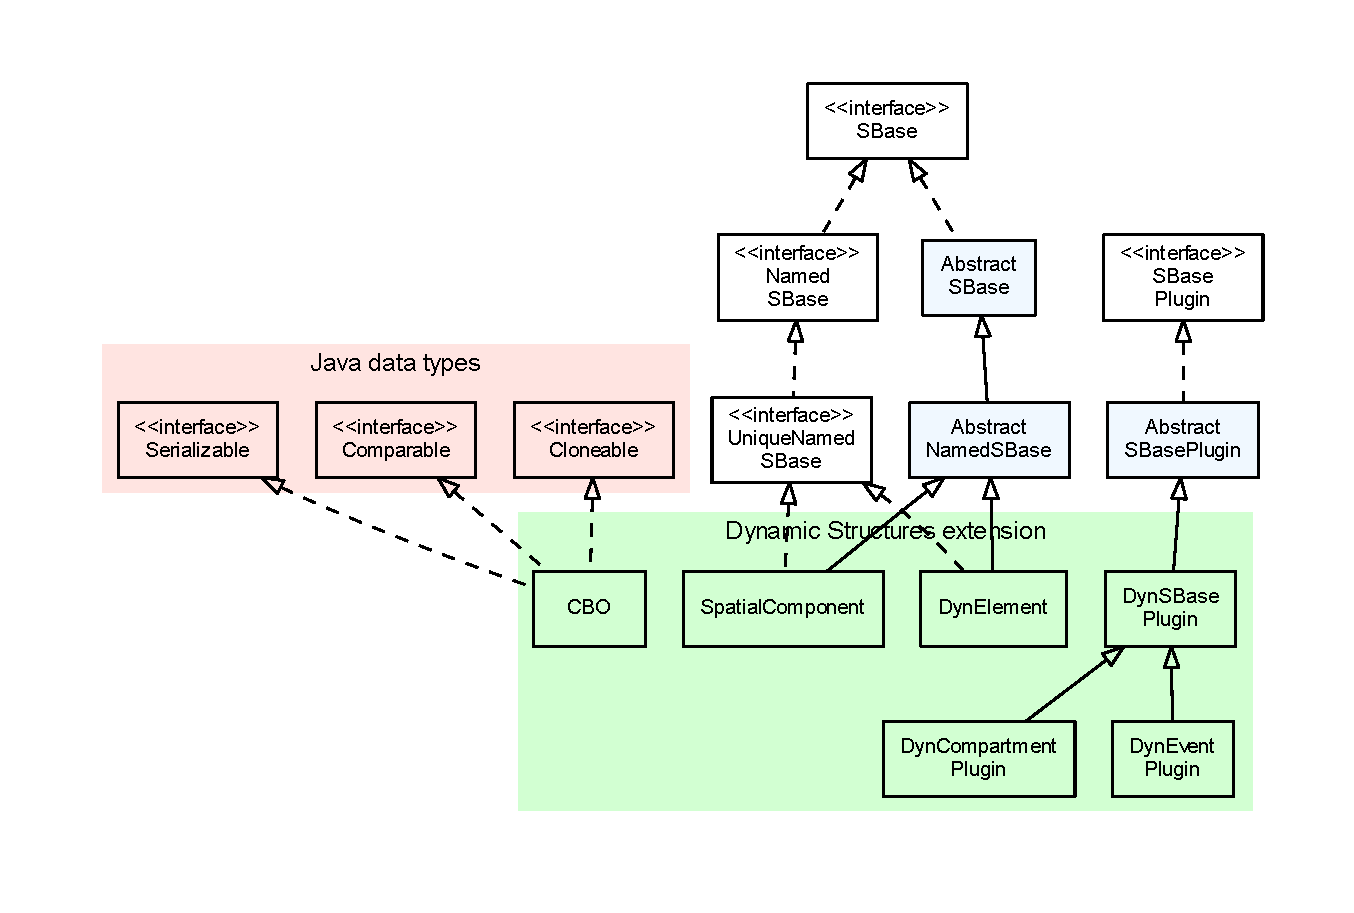
\includegraphics[width=\textwidth]{../../../extensions/dyn/doc/img/type_hierarchy.pdf}
 \caption[Class diagram of the dynamic structures extension]{Class diagram of the dynamic structures extension. Dynamic Structures (\code{dyn}, \cite{Gomez2014}), supports the definition of dynamical behaviors for model entities.
}
 \label{fig:dyn}
\end{figure}


\begin{figure}[hb]
 \centering
 \vspace*{2ex}
 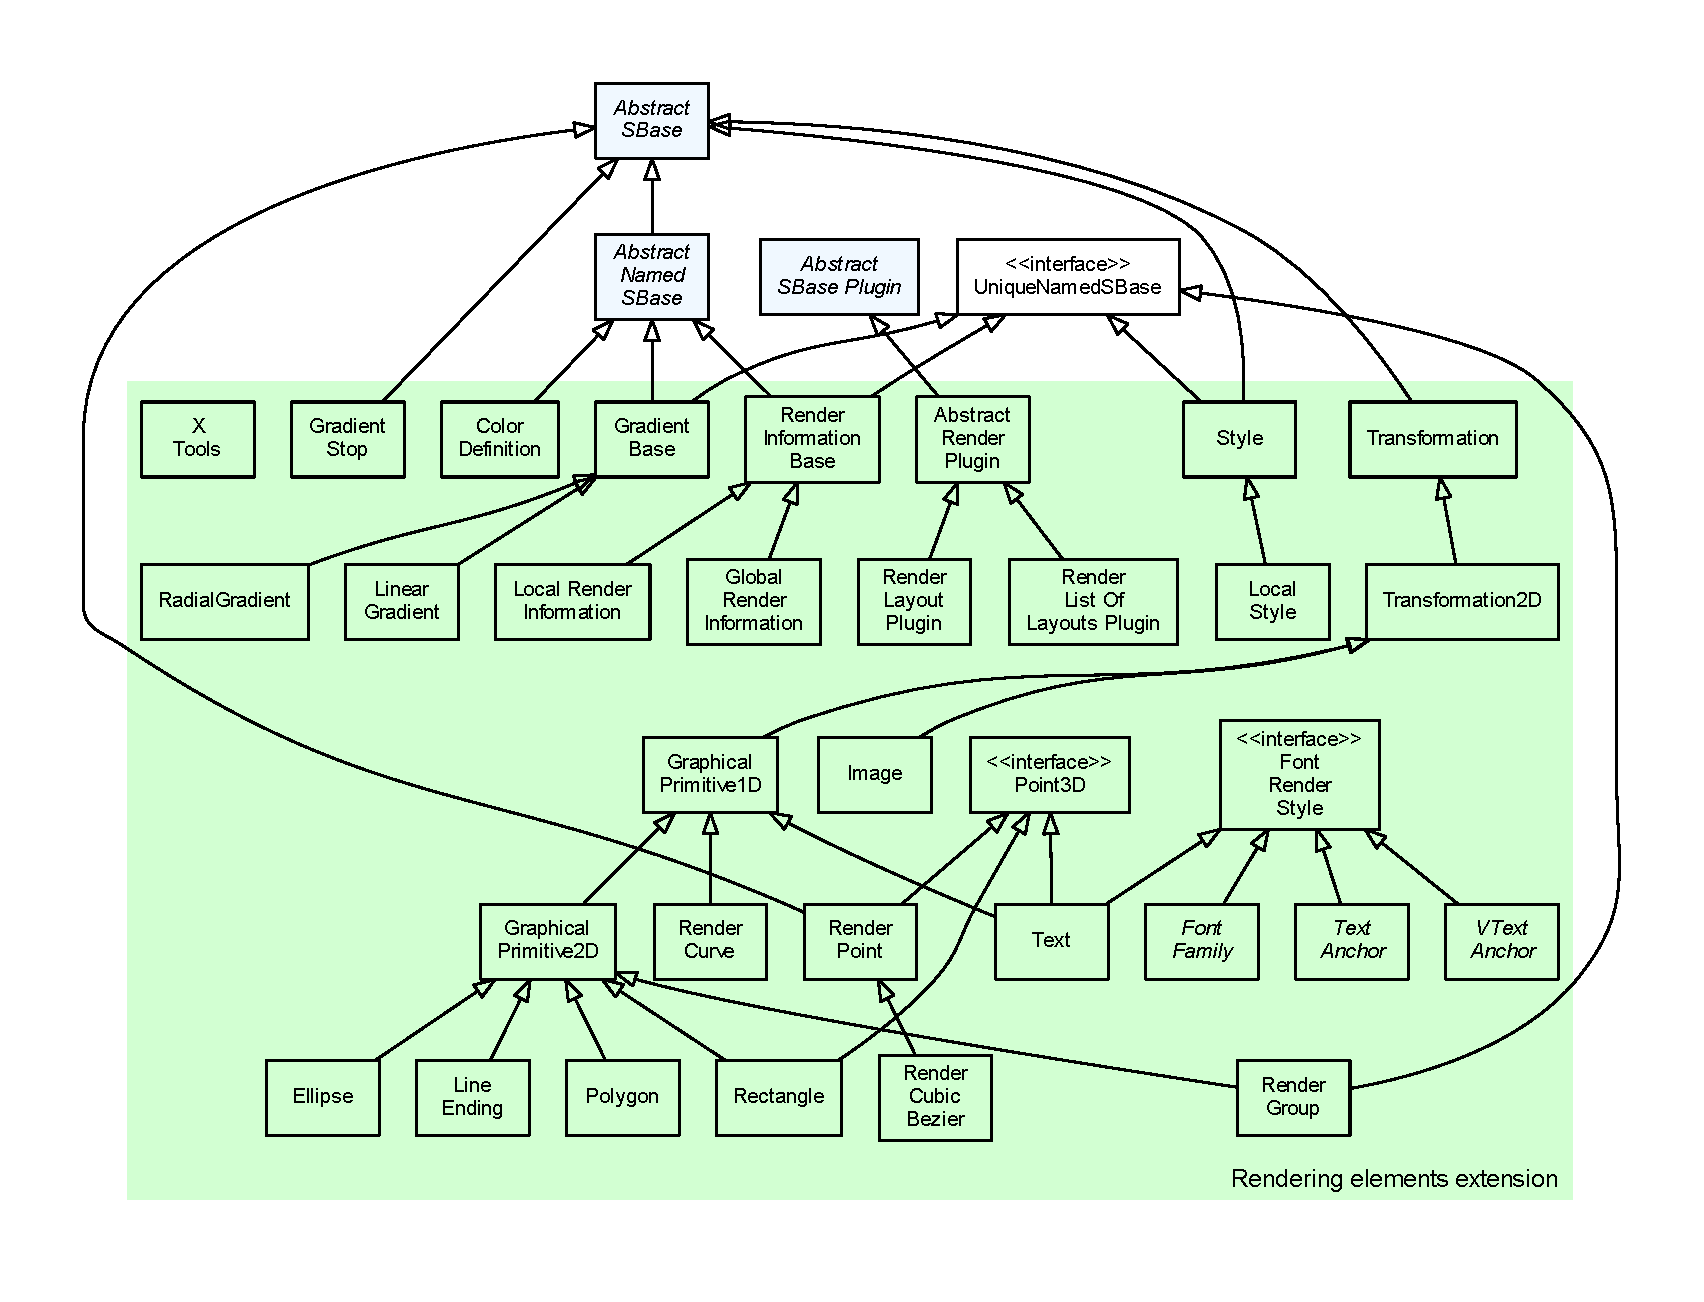
\includegraphics[width=\textwidth]{../../../extensions/render/doc/img/type_hierarchy.pdf}
 \caption[Class diagram of the rendering extension.]{Class diagram of the rendering extension. Rendering (\code{render}, \cite{gauges2006}) couples with \cite{Layout} to provide symbol and style information for network diagrams.}
 \label{fig:render}
\end{figure}


